\begin{tikzpicture}[overlay, remember picture]
    \node[anchor=north west, rotate=0, gray, font=\tiny, text width=\paperwidth] at (current page.south west)  [xshift=0, yshift=1.25cm] {
    [1] L. Amico et al., Entanglement in Many-Body Systems, Reviews of Modern Physics 80, no. 2 (2008)

    [2] A. Bergschneider et al., Experimental Characterization of Two-Particle Entanglement through Position and Momentum Correlations, Nature Physics 15, no. 7 (2019)
    };
\end{tikzpicture}

\only<1>{
\vspace{-7mm}
We can measure correlations: \vspace{-2mm}
\begin{figure}[h]
    \centering
    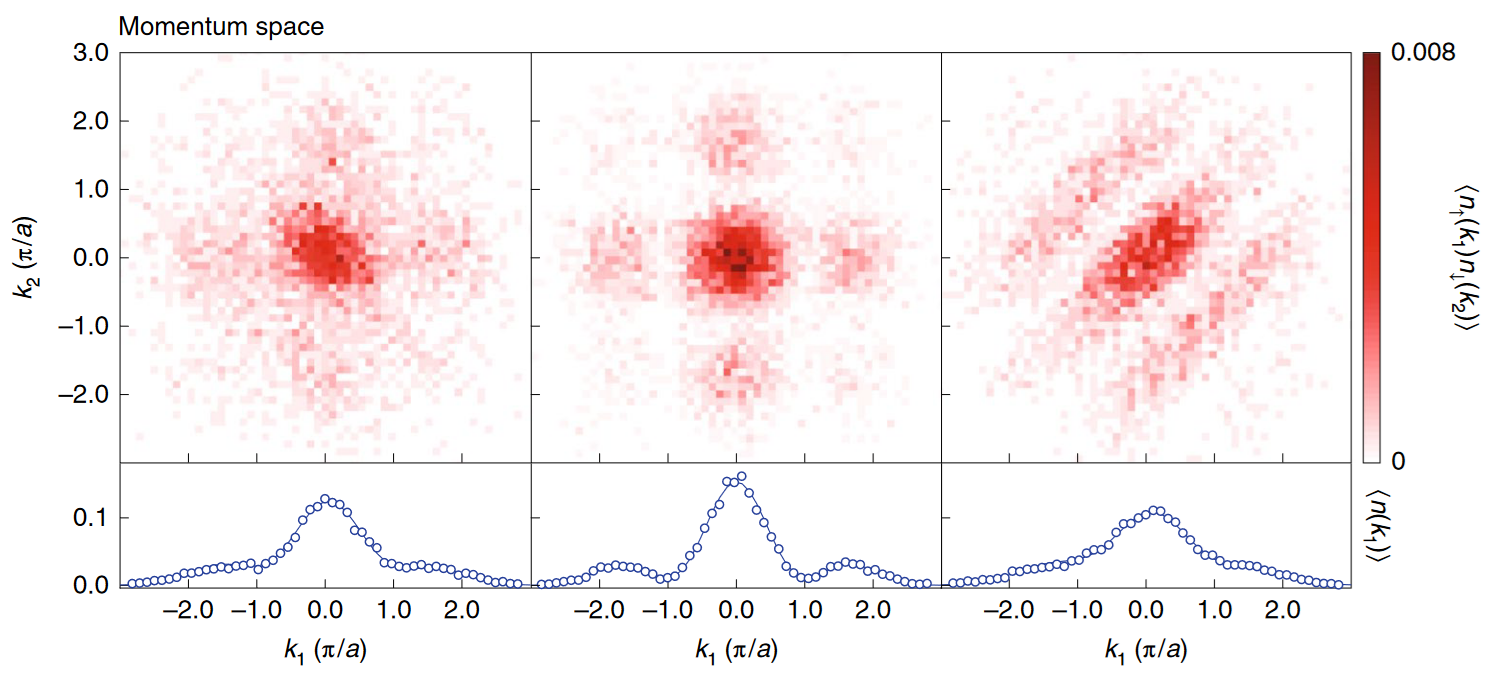
\includegraphics[width=0.75\textwidth]{imgs/eexp1.png}
    %\caption{}
    %\label{fig:}
\end{figure}
}

\only<2>{
\vspace{-7mm}
The pair correlators as entanglement witnesses: \vspace{-2mm}
    \begin{figure}[h]
        \centering
        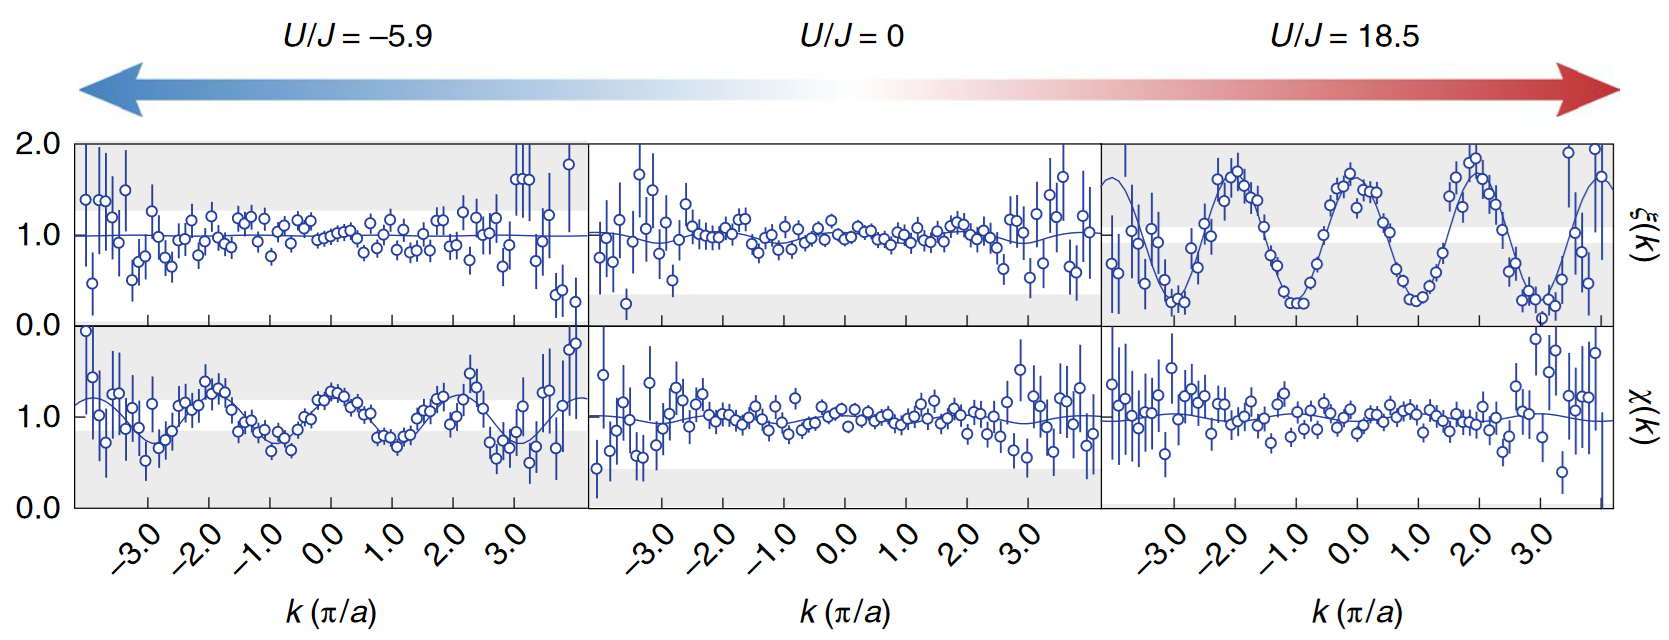
\includegraphics[width=0.9\textwidth]{imgs/eexp2.png}
        %\caption{}
        %\label{fig:}
    \end{figure}
    
}

\only<1>{
Construct the pair correlators \vspace{-3mm}
\begin{align*}
    \xi(d=k_1-k_2) &= \frac{
        \int d k\ \langle n_{\uparrow}(k-d/2) n_{\downarrow}(k+d/2)\rangle
    }{
        \int d k\ \langle n_{\uparrow}(k-d/2) \rangle \langle n_{\downarrow}(k+d/2)\rangle
    } 
    \\
    \chi(s=k_1+k_2) &= \frac{
        \int d k\ \langle n_{\uparrow}(k+s/2) n_{\downarrow}(-k+s/2)\rangle
    }{
        \int d k\ \langle n_{\uparrow}(k+s/2) \rangle \langle n_{\downarrow}(-k+s/2)\rangle
    } 
\end{align*}
}

\only<2>{

\phantom{42}

    For separable states: \vspace{-3mm}
    \begin{equation*}
         \sub{\xi}{min} \leq \xi  \leq \sub{\xi}{max},
         \hspace{5 mm} 
         \sub{\chi}{min} \leq \chi  \leq \sub{\chi}{max}.
    \end{equation*}
}
